\documentclass[12pt,a4paper,titlepage]{article}
\usepackage[utf8]{inputenc}
\usepackage{lmodern}
\usepackage[T1]{fontenc}
\usepackage{epsfig}
\usepackage{listings}
\usepackage{graphicx}
%\usepackage{underscore}
\usepackage{amsmath}
\usepackage{textcomp}
\usepackage[unicode,breaklinks=true,hypertexnames=false]{hyperref}	
\numberwithin{equation}{subsection}


%\title{TB2 manual}
%\author{ROBO@FIT}
%\date{\today}


\begin{document}

%\maketitle

\begin{titlepage}

\begin{center}

 \begin{figure}
	\centering
\includegraphics[width=3cm]{./img/robot.pdf}
 \end{figure}
 
\vspace*{100pt}

% Title
\rule{\linewidth}{0.5mm}

{ \vspace{15pt} \huge \bfseries TB2 manual}
\vspace{15pt}
\rule{\linewidth}{0.5mm}

\vspace{50pt}

\textsc{\Large \bfseries ROBO@FIT}


\vspace{30pt}
\large \today


\end{center}

\end{titlepage}

\begin{abstract}
TB2 is an indoor robotic platform running ROS. It offers suite of the most common sensors, basic manipulator and quite long battery life. It's suitable for testing navigation, mapping, perception and manipulation algorithms.

\begin{center}
 \begin{figure}
	\centering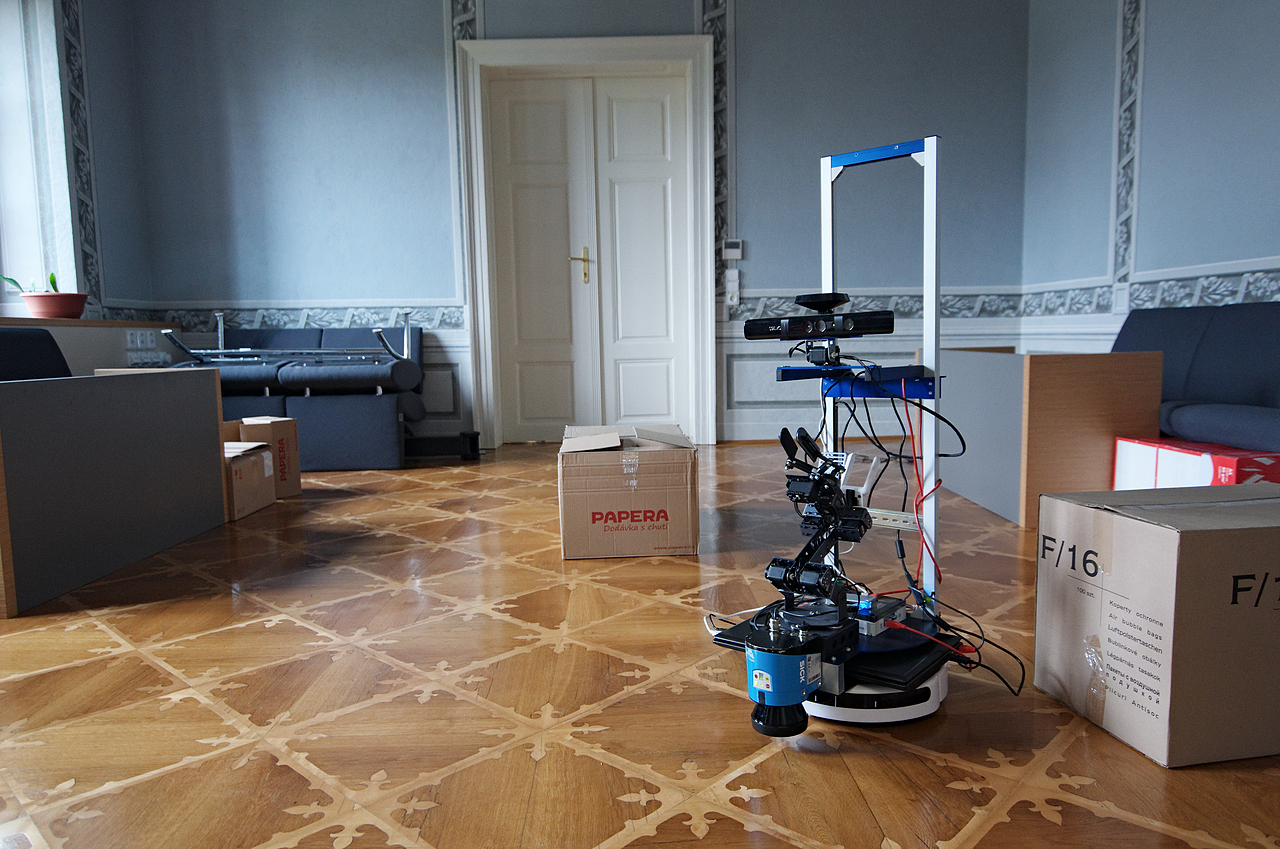
\includegraphics[width=15cm]{./img/DSC_1746.jpg}
 \end{figure}
\end{center}

\end{abstract}

\tableofcontents % create a table of content

\newpage

% ---------------------------------------------------------------------------
% ---------------------------------------------------------------------------
\section{Hardware overview}

TB2 is inspired by Turtlebot which is de facto standard low-cost robotic platform. Unlike original Turtlebot, TB2 has more sensors, manipulator and much more battery life.

\begin{center}
 \begin{figure}
	\centering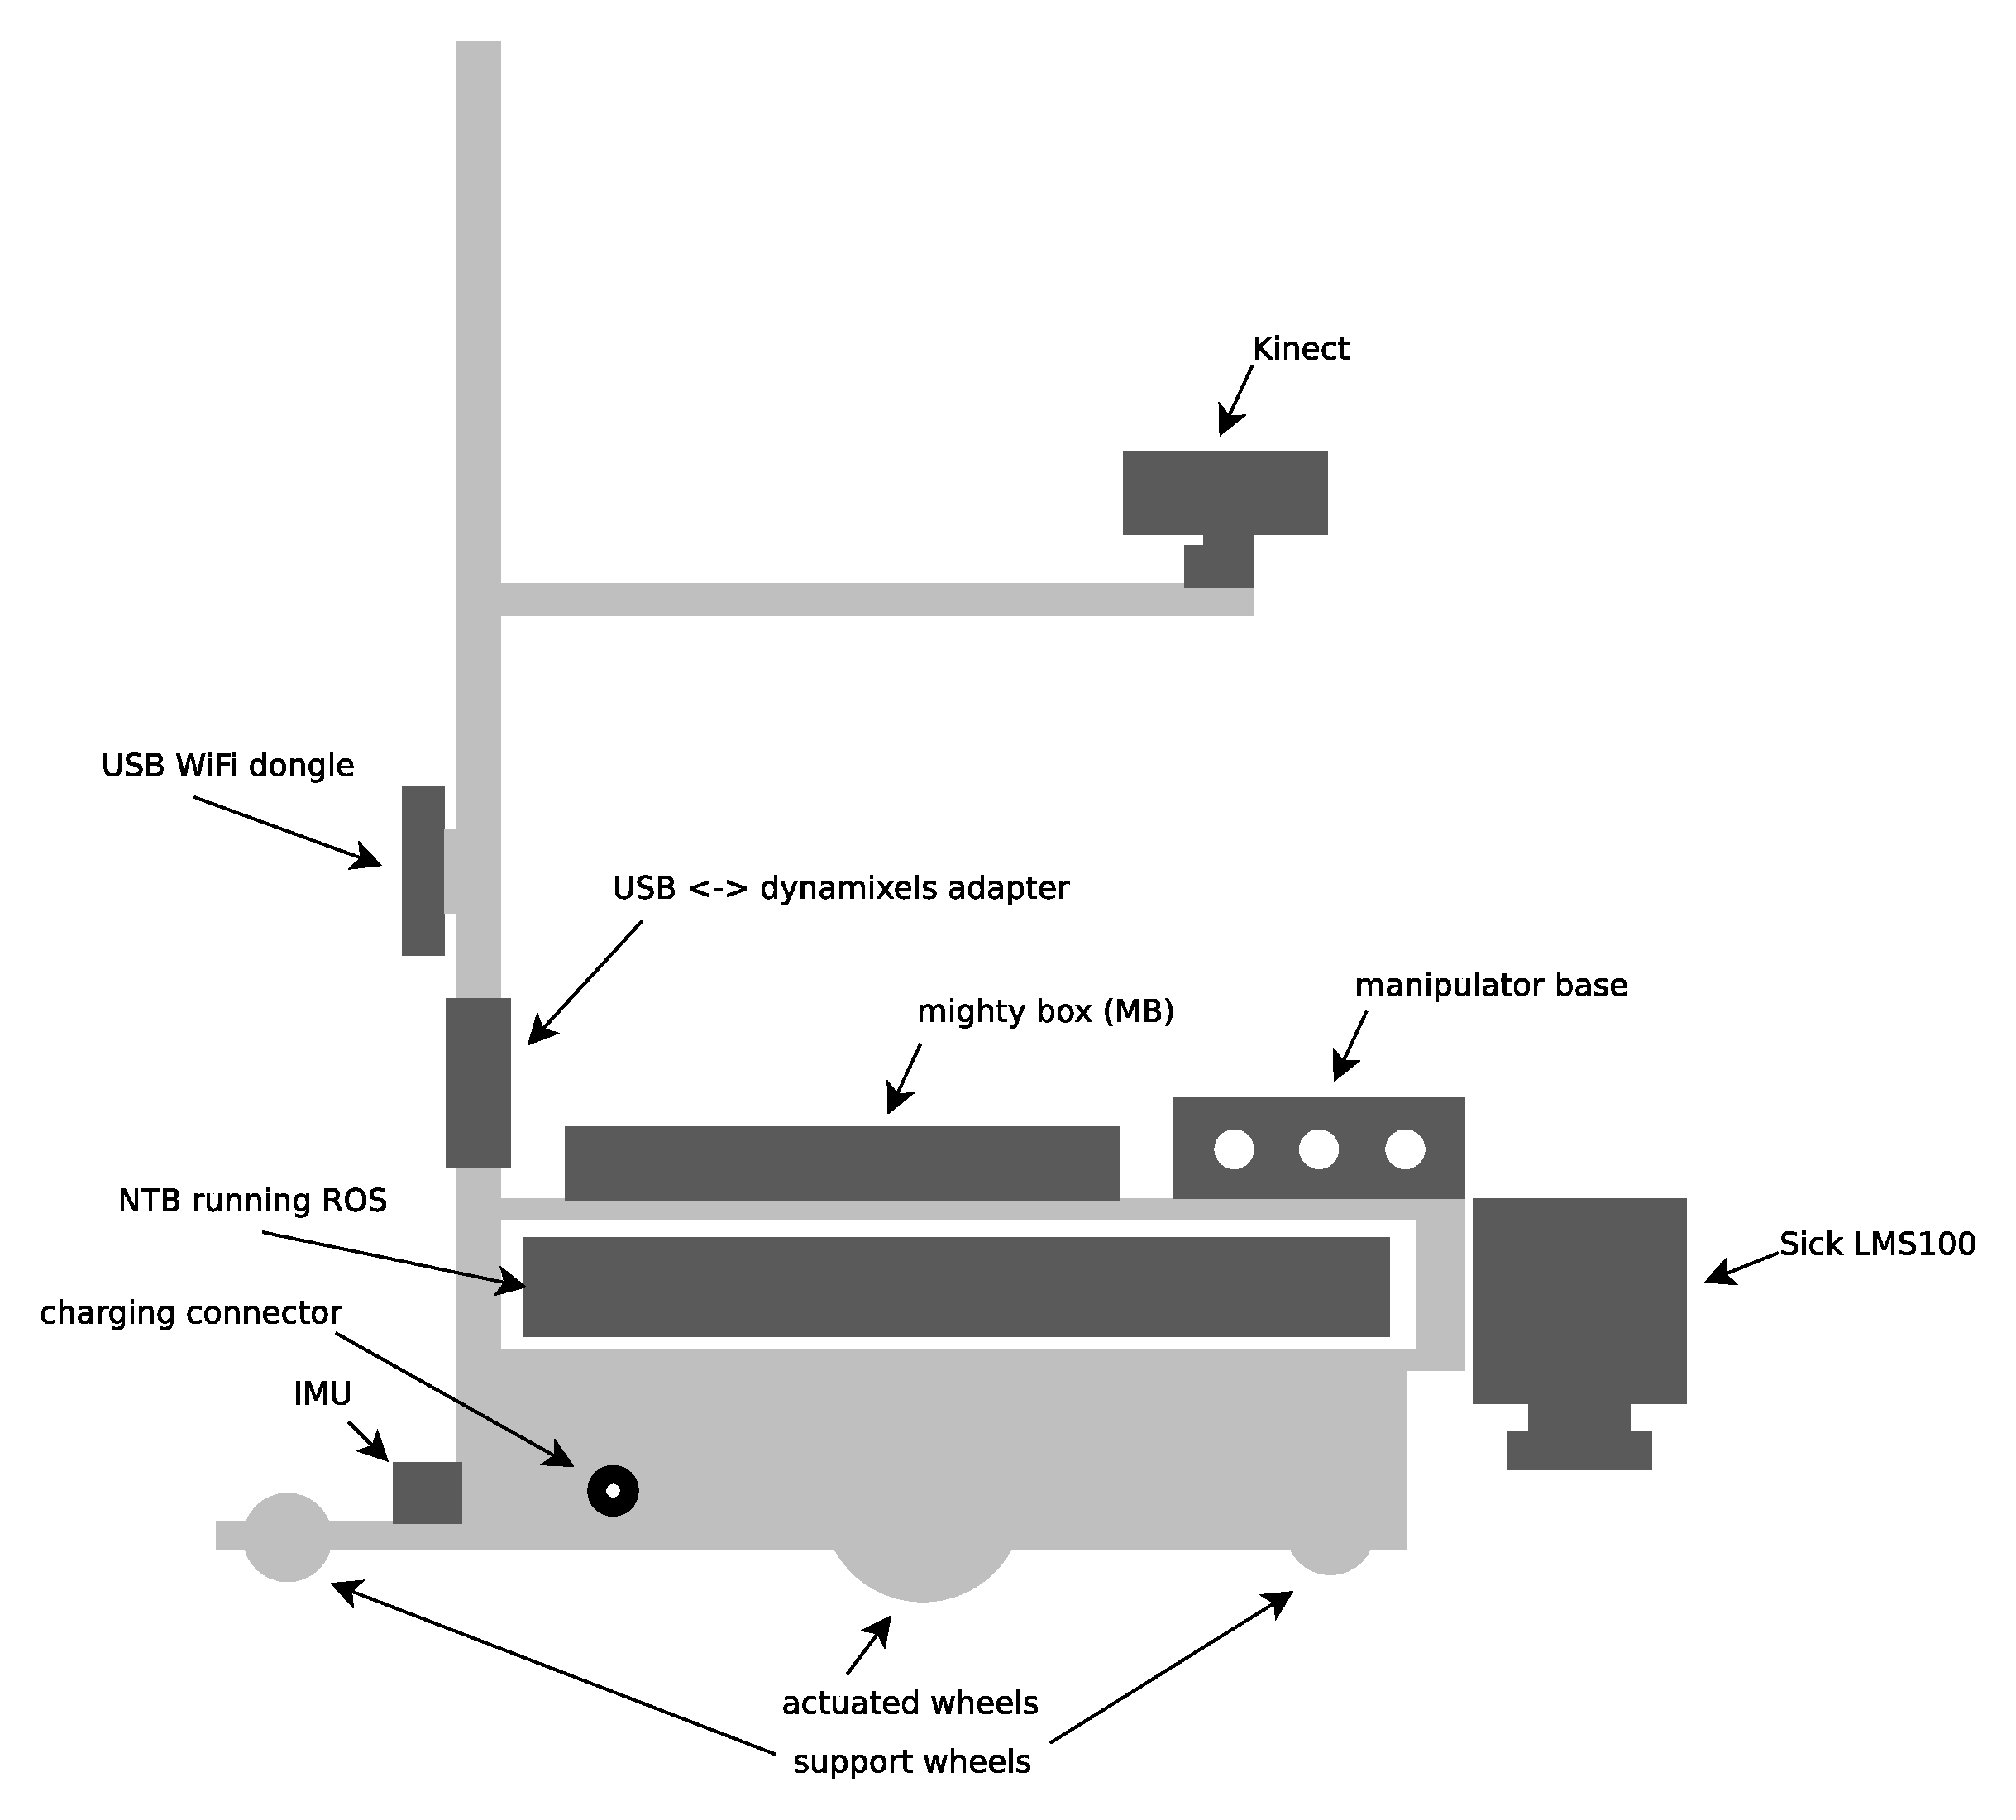
\includegraphics[width=16cm]{./img/tb2.pdf}
 \caption{Schematic image of TB2 from right side.}
 \label{fig:tb2}
 \end{figure}
\end{center}

\subsection{Base}

Base of the robot is modified iRobot Roomba 530 (all cleaning stuff has been removed).
Any Roomba can be commanded using special port which is normally hidden by top cover. It's ordinary serial port, but in TTL levels (+5~V). This interface is called \href{http://www.irobot.com/images/consumer/hacker/roomba_sci_spec_manual.pdf}{Serial Command Interface (SCI)} and can be used to control motors and read state of all sensors.

\begin{center}
 \begin{figure}[!h]
	\centering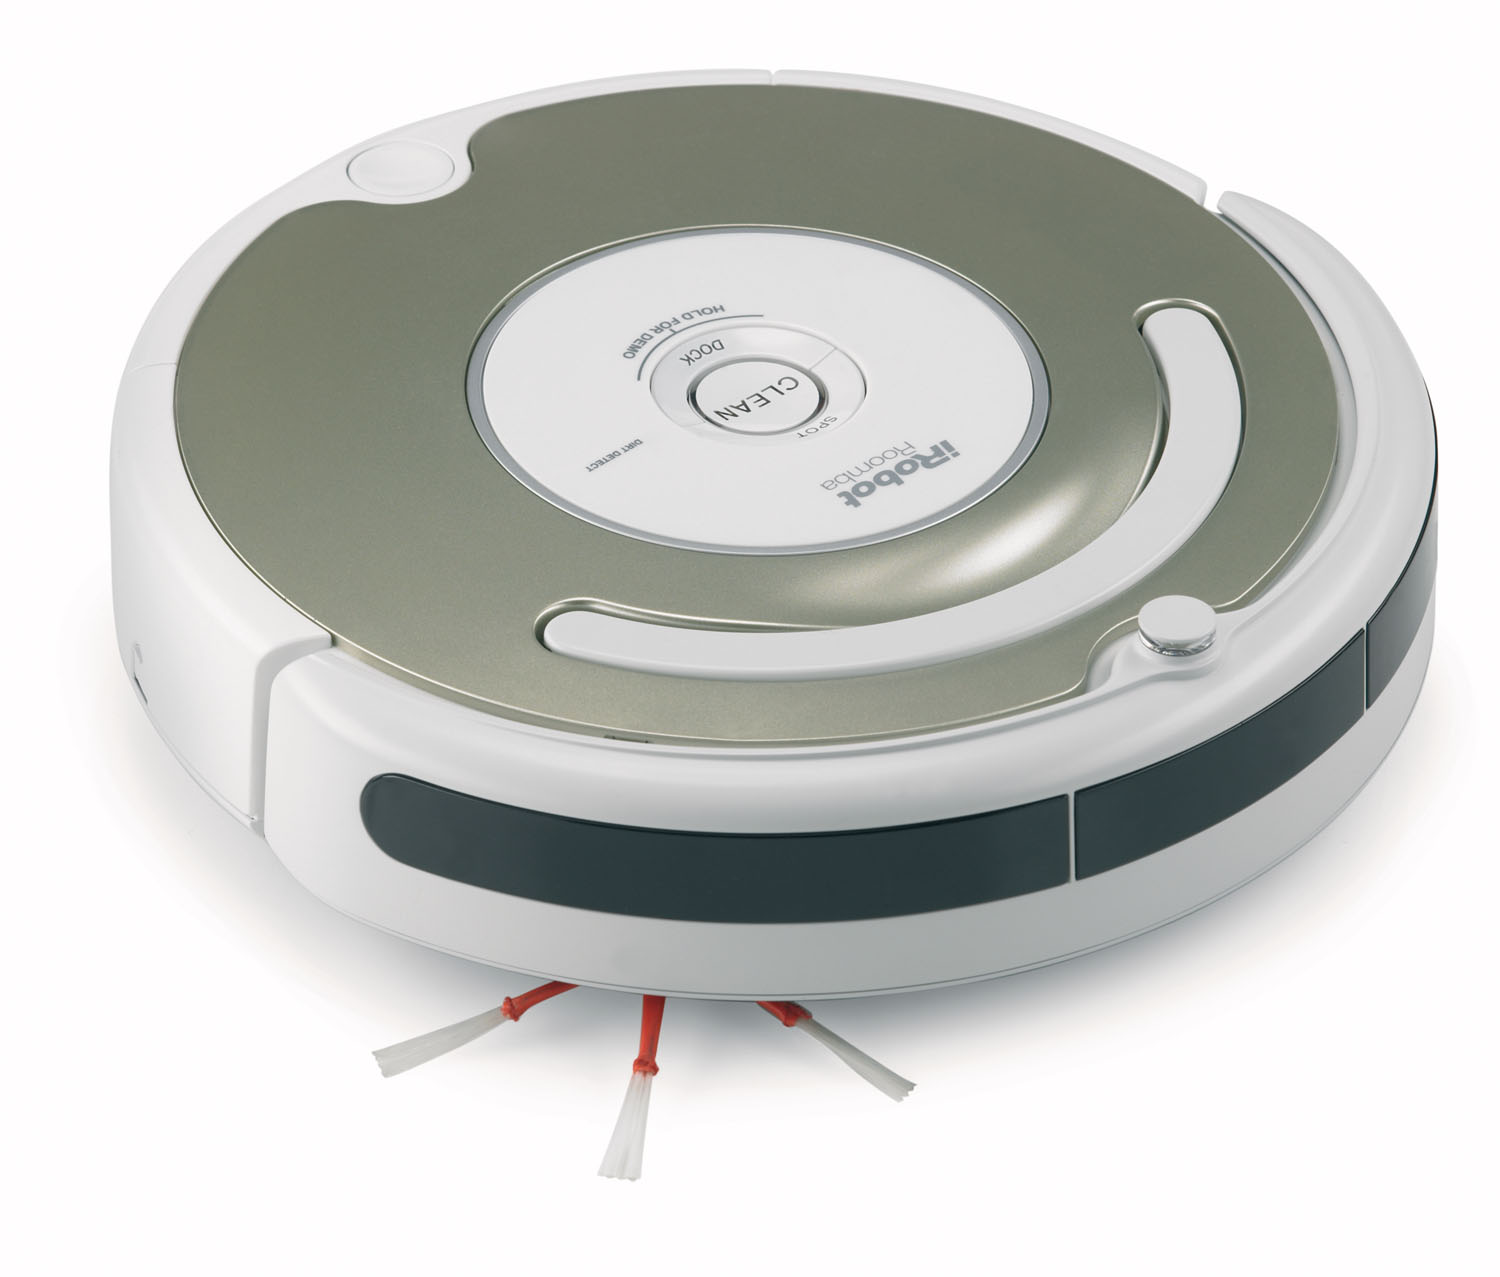
\includegraphics[width=6cm]{./img/roomba-530.jpg}
 \caption{iRobot Roomba 530.}
 \label{fig:roomba}
 \end{figure}
\end{center}

Buttons of Roomba are accesible on top blue plate. Red one will switch Roomba ON. Long press of red button will switch base OFF. Simultaneous press of two black buttons will reset base\footnote{This might be the case if you have problems to bring up robot.}.

\subsection{Power sources}

Base has it's own separate battery. Other sensors and actuators are powered from Li-On batteries (white blocks visible from back side of the robot). Bigger battery (8,8~Ah) is usually used for powering manipulator and smaller (6,6~Ah) for powering sensors. Batteries are connected to MB with green female push-on connector.

It's possible to swap batteries to provide more battery life to sensors instead of arm. In case of need, please ask boss (\ref{sec:notes}) of the TB2.

\subsection{Mighty box}

As you can see on Figure \ref{fig:tb2}, there is some "mighty box" (MB). It can be switched on by pressing \emph{ON/OFF} button - then you shoud see \emph{LED1} and \emph{LED2} shining. Press \emph{ON/OFF} button for at least three seconds to shut it down.

This MB is connected to NTB by USB~2.0 device connector and acts as USB to serial converter for base (USB device connector labeled \emph{NTB}), two IMUs (\emph{IMU1} and \emph{IMU2}) and internal microprocessor. Activity on these serial links is indicated by LEDs \emph{ROB}, \emph{IMU1}, \emph{IMU2} and \emph{uP}. If MB is the first connected USB to serial converter to your PC (and it should be!) you will find this devices in your /dev directory:

\begin{itemize}
  \item{/dev/ttyUSB0 - Roomba}
  \item{/dev/ttyUSB1 - right IMU}
  \item{/dev/ttyUSB2 - left IMU}
  \item{/dev/ttyUSB3 - MB's internal microprocessor}
\end{itemize}

MB also has some power circuitry to provide +12~V power to sensors (Kinect, laser scanner) from Li-On batteries. On the same side as \emph{NTB} connector, there are also two USBs which can be used to provide some additional power to devices like external HDD etc.

Internal microprocessor is monitoring state of all baterries and sending this state through serial port in ASCII form. How to see it:

\begin{itemize}
  \item{open serial terminal program (e.g. cutecom)}
  \item{open /dev/ttyUSB3, at 19200 baud}
  \item{you will see output like this: \#BS: 16,5V, BA: 16,6V, BR: : 13,5V}
  \item{BS means sensors battery (Li-On), BA arm battery (Li-On) and BR robot's internal battery (Ni-Mh)}
\end{itemize}

State of Li-On batteries is also indicated by blinking LEDs on the board (they are named \emph{BAT-ARM} and \emph{BAT-SEN}). Shorter flash of LED means lower voltage. In case of critical low voltage on any of two batteries MB will shutdown.

\subsection{Sensors}

On top of TB2 there is \href{http://en.wikipedia.org/wiki/Kinect}{Microsoft Kinect} which is able to produce RGBD images with 640x480 pixels at 30~Hz. It's connected to notebook using USB 2.0 and powered from MB.

Front side of TB2 is eqquiped with \href{http://en.wikipedia.org/wiki/LIDAR}{laser scanner}, namely \href{http://www.sick.com/us/en-us/home/products/product_news/laser_measurement_systems/Pages/lms100.aspx}{Sick LMS100}. It has 270\textdegree{} field of view with resolution of 0.5\textdegree{}, range up to 20~meters and scanning frequency 50~Hz. It's powered from MB \footnote{After switching MB on, scanner needs some time to initialize.} and connected to NTB by Ethernet.

TB2 has also two inertial measurements units (IMU). It's \href{http://www.chrobotics.com/docs/UM6_datasheet.pdf}{CH Robotics UM6} which combines gyro, accelerometer, magnetic sensor and provides orientation at up-to 500~Hz rate. 

\subsection{Manipulator}

\href{http://crustcrawler.com/products/AX-18F\%20Smart\%20Robotic\%20Arm/}{CrustCrawler AX-18A Smart Robotic Arm}.

\emph{TODO - add some description.}


\subsection{Charging}

Charging of the base using docking station is not possible because of laser scanner mounted on front side of robot. However there is charging connector on right side of base, see \ref{fig:tb2}. During charging, the LEDs in the middle of the base (under the notebook) are blinking and they become green when the base is fully charged. Original Roomba has one Ni-Mh battery with 3000~mAh capacity, TB2 has two these batteries. It means longer battery life, but also longer charging with standard Roomba charger. Because the capacity of batteries is quite high, it's NOT neccesary to charge them each day, before each usage of robot.

For charging manipulator and sensor's battery you will need dual DC power supply \ref{fig:dc-supply} and special cable\footnote{That special cable is usualy connected to DC power supply at robot's office.}. Switch DC supply on, set both voltages to 16,7~V and set maximum current (around 3,5~A). Disconnect green female connector of batteries from MB and connect it to that special cable. Batteries are charged when the charging current is approximately zero amperes. These Li-On batteries can be charged at any time.

\begin{center}
 \begin{figure}[!h]
	\centering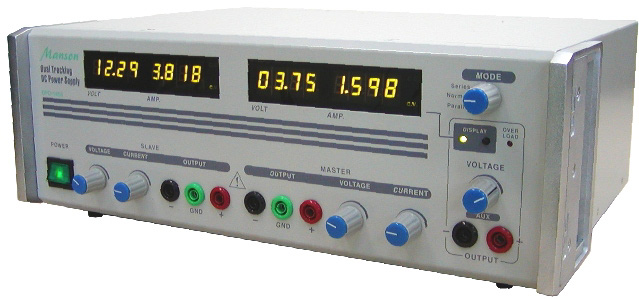
\includegraphics[width=6cm]{./img/dc-supply.jpg}
 \caption{Dual DC power supply.}
 \label{fig:dc-supply}
 \end{figure}
\end{center}

\subsection{Networking}

TB2 network consists of wireless router (current one is TP-LINK TL-WR1043ND), robot (NTB with external wifi dongle) and some operator (you).

\begin{center}
 \begin{figure}[h]
	\centering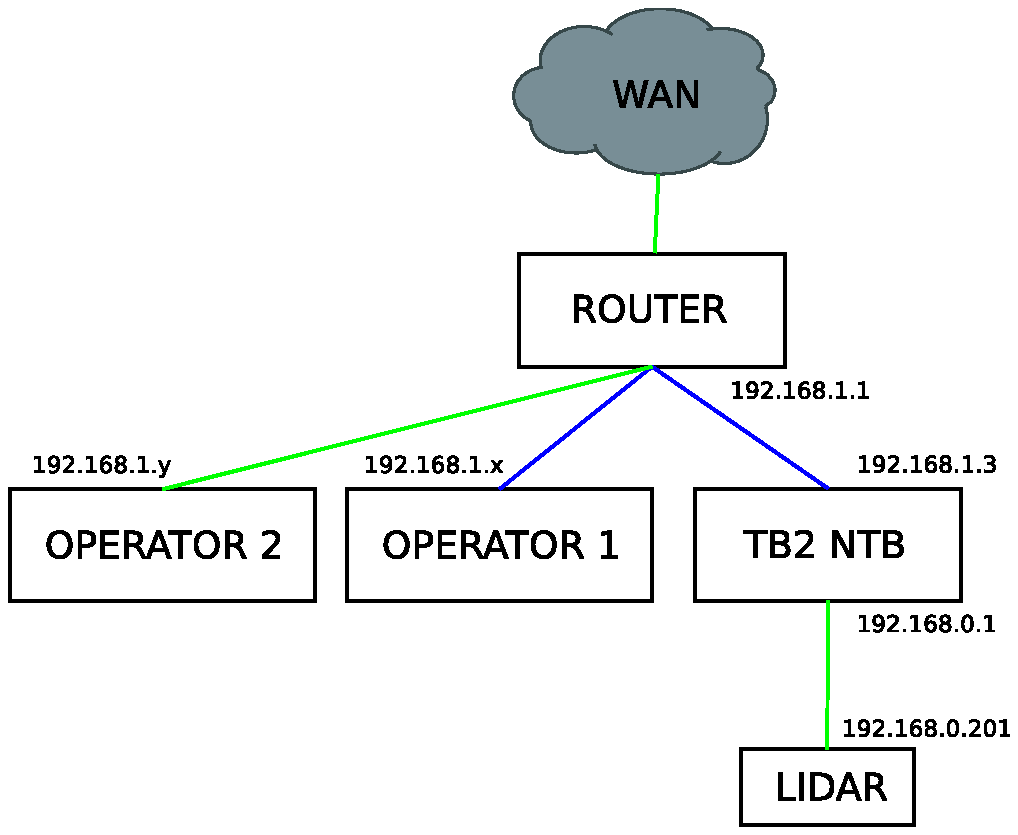
\includegraphics[width=10cm]{./img/networking.pdf}
 \caption{TB2 network. Green line means wired connection and blue wireless.}
 \label{fig:tb2-networking}
 \end{figure}
\end{center}

Robot is always connected to router using WiFi and it always has address 192.168.1.3, but there is DNS working, so one can use just it's name (\verb|turtlebot|). Router offers N network with speed up to 300~Mbps. Current speed can be checked with \verb|ifconfig| command. Operator can connect to router with cable (preffered way) or using WiFi. Of course, router can be connected to internet and then robot and operator will have access to it too.

Router's wireless network is called "turtlebot" and password is same as router's pin (printed on bottom side of router).

%\newpage
% ---------------------------------------------------------------------------
% ---------------------------------------------------------------------------
\section{Software overview}

Robot is currently running on \href{http://ros.org/wiki/electric}{ROS Electric}.

If you want to use real robot, it's fine just to use robot's notebook and connect to it remotely with any PC. There is no need to install anything on your machine. If you want to run simulation, you will probably need to install almost everything because many components are needed for real as well as for simulated robot\footnote{It would be nice to divide packages and installation instructions for use with real or with simulated robot. Any voluntier?}.

\subsection{Installation}

As the robot is running ROS Electric you will need Ubuntu 11.04 or 11.10. Follow \href{http://www.ros.org/wiki/electric/Installation/Ubuntu}{installation procedure}. It's highly recomended to use precompiled Debian packages.

Run this command to install all needed dependencies from ROS repository:

\begin{verbatim}
sudo apt-get install ros-electric-cob-environments
ros-electric-dynamixel-motor ros-electric-image-transport-plugins
ros-electric-pr2-controllers ros-electric-pr2-mechanism
ros-electric-joystick-drivers ros-electric-navigation
ros-electric-openni-kinect ros-electric-robot-model
ros-electric-simulator-gazebo ros-electric-turtlebot-apps
ros-electric-turtlebot-viz ros-electric-vision-opencv
ros-electric-turtlebot-simulator ros-electric-cob-simulation
ros-electric-image-common
\end{verbatim}

Then, checkout following repositories\footnote{This instalation procedure (including complete commands) can be also found in \emph{README.txt} in \emph{tb2\_main\_packages} stack.} to directory in your ROS\_PACKAGE\_PATH using SVN (\verb|svn co repo|):

\begin{itemize}
  \item{\href{http://aptima-ros-pkg.googlecode.com/svn/trunk/imu_um6}{IMU driver}}
  \item{\href{http://ua-ros-pkg.googlecode.com/svn/trunk/arrg/crustcrawler_smart_arm/}{manipulator description}}
  \item{\href{http://isr-uc-ros-pkg.googlecode.com/svn/stacks/serial_communication/trunk/}{driver for Roomba}}
\end{itemize}

And these using git (\verb|git clone|):

\begin{itemize}
  \item{\href{git://github.com/konradb3/RCPRG-ros-pkg.git}{LMS100 driver}}
  \item{\href{https://github.com/ccny-ros-pkg/scan_tools.git}{laser\_scan\_matcher package}}
\end{itemize}

It might be necessary to run also this command

\begin{verbatim}
rosdep install scan_tools
\end{verbatim}

If you want to run real robot, it will be necessary to patch LMS100 driver. Switch to \verb|LMX1xx| package, open \verb|LMS1xx_node.cpp| and:

\begin{itemize}
 \item{find line 55 "num\_values = 541;"}
 \item{and line 59 "num\_values = 1081;"}
 \item{swap values}
\end{itemize}

Now you can try to build all TB2 packages:

\begin{verbatim}
roscd tb2_main_packages
rosmake
\end{verbatim}

If you want to use only simulation, you can put \verb|ROS_NOBUILD| file to packages which are not needed for simulation and then compile other packages:

\begin{verbatim}
roscd btb_base_driver; touch ROS_NOBUILD
roscd btb_bringup; touch ROS_NOBUILD
roscd btb_imu; touch ROS_NOBUILD
roscd btb_dynamixel; touch ROS_NOBUILD
roscd tb2_main_packages
rosmake
\end{verbatim}

\subsection{Brief description of packages}

\begin{itemize}
 \item{btb\_assisted\_arm\_navigation $\rightarrow$ TB2's version of \href{http://ros.org/wiki/srs_assisted_arm_navigation}{srs\_assisted\_arm\_navigation}}
 \item{btb\_base\_driver $\rightarrow$ improved version of Roomba driver}
 \item{btb\_bringup $\rightarrow$ start real robot}
 \item{btb\_common $\rightarrow$ RVIZ launch file etc.}
 \item{btb\_description $\rightarrow$ URDF files}
 \item{btb\_dynamixel $\rightarrow$ configuration, launch files and scripts for manipulator}
 \item{btb\_exploration $\rightarrow$ for exploring unknown area using (to be used with SLAM)}
 \item{btb\_gazebo $\rightarrow$ simulation of TB2}
 \item{btb\_imu $\rightarrow$ driver and launch files for IMU}
 \item{btb\_manipulator $\rightarrow$ arm\_navigation stack related stuff}
 \item{btb\_manipulator\_openrave $\rightarrow$ openrave related stuff}
 \item{btb\_navigation $\rightarrow$ SLAM, localization}
 \item{btb\_teleop $\rightarrow$ for manual control}
\end{itemize}


\subsection{Running simulation}

For properly running simulation, it's better to NOT have ROS installed on system inside VirtualBox or another virtualization tool. It's also recomended to have NVIDIA graphics card.

You can run just robot in empty world:

\begin{verbatim}
roslaunch btb_gazebo robot_empty_world.launch
\end{verbatim}

or you can have robot in some non-empty environment:

\begin{verbatim}
roslaunch btb_gazebo robot_wg_world.launch
\end{verbatim}

When using TB2 notebook for running simulation, add \verb|optirun| before \verb|roslaunch|, otherwise Gazebo will not use NVIDIA card.

There are more worlds available, please check launch files in \verb|btb_gazebo| package\footnote{Selection of world should be done by change of environment variable, but this feature is not ready yet. Any voluntier?}.

\begin{center}
 \begin{figure}[h]
	\centering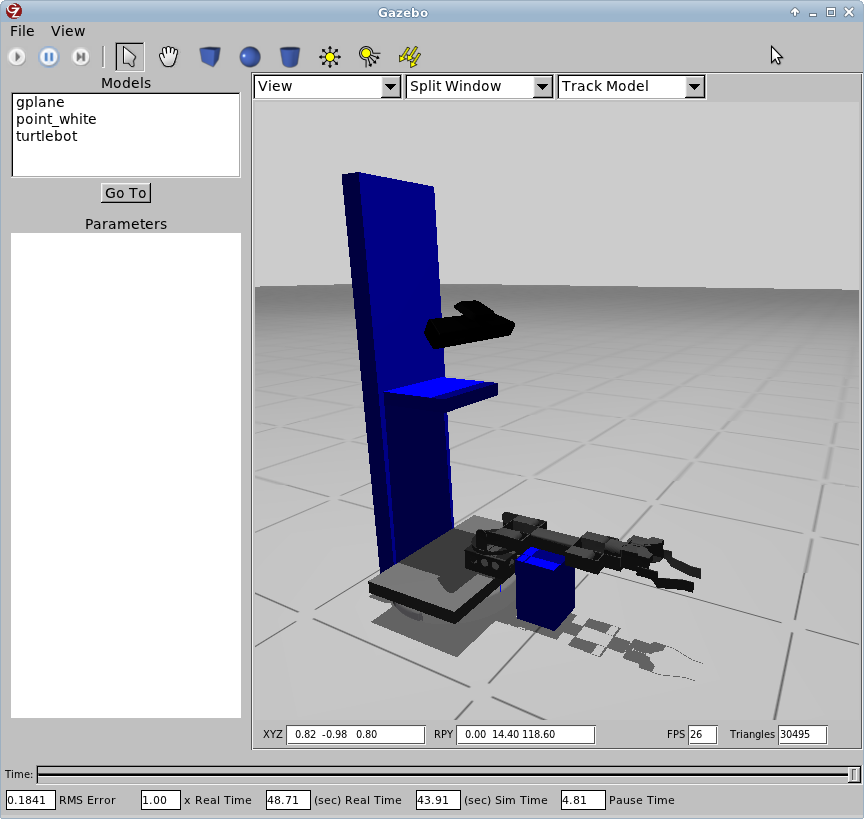
\includegraphics[width=10cm]{./img/tb2-gazebo.png}
 \caption{TB2 simulated in Gazebo.}
 \label{fig:tb2-gazebo}
 \end{figure}
\end{center}

\emph{TODO - describe basic differences between the simulated and the real TB2 - some topics are available only on one of them etc.}


\subsection{Teleoperation}

There are more ways how to remotely control robot.

Teleoperation using keyboard on local machine:

\begin{verbatim}
export ROS_MASTER_URI=http://turtlebot:11311
roslaunch btb_teleop keyboard_teleop.launch
\end{verbatim}

or using remote shell:

\begin{verbatim}
ssh fit@turtlebot
roslaunch btb_teleop keyboard_teleop.launch
\end{verbatim}

Another posibility is to use interactive teleop (which is started automatically with simulated or real robot) or PS3 gamepad - see \ref{sec:robot-usage}.

\emph{TODO - add screenshot of RVIZ teleop and some desc.}

\subsection{Navigation}

Running SLAM:

\begin{verbatim}
roslaunch btb_navigation laser_gmapping_demo.launch
\end{verbatim}

Running localization:

\begin{verbatim}
export ROBOT_ENV=ipa-apartment
roslaunch btb_navigation laser_amcl_demo.launch
\end{verbatim}

Already prepared environments:

\begin{itemize}
 \item{ipa-apartment}
 \item{ipa-kitchen}
 \item{willow}
\end{itemize}


\subsection{Using manipulator}

\emph{TODO - topics, services, move\_arm action, assisted arm navigation (control of arm using RVIZ), closing/openning gripper.}

%\newpage
% ---------------------------------------------------------------------------
% ---------------------------------------------------------------------------
\section{Robot usage}
\label{sec:robot-usage}

Some notes about practical robot usage.

\subsection{Remote access}

Notes: username of \verb|fit| user is \verb|upgm|.

Remote desktop using VNC, for instance Remmina client.

Remote shell using ssh:

\begin{verbatim}
ssh -X -C fit@turtlebot
\end{verbatim}

Starting RVIZ (or any other node) locally:

\begin{verbatim}
export ROS_MASTER_URI=http://turtlebot:11311
rosrun rviz rviz
\end{verbatim}

\subsection{Starting robot}

When starting robot, please follow these steps:

\begin{itemize}
  \item{plug wifi USB dongle into robot's NTB (on the left side of NTB)}
  \item{make sure you can connect remotely to robot}
  \item{put NTB into robot}
  \item{switch on MB}
  \item{connect black USB (from MB) to hub, then white one (USB dynamixel converter)}
  \item{connect hub to NTB}
  \item{plug laser scanner Ethernet cable to NTB}
  \item{using remote desktop, connect to laser network}
  \item{switch on Roomba by pressing red button}
  \item{in one terminal tab, run \verb|roscore| and in another \verb|rxconsole|}
  \item{run \verb|roslaunch btb_bringup robot.launch|}
\end{itemize}

Robot should move a little bit. Then it's fine. If it will not move, it will try to initialize base again in 45 seconds. In meantime, press red button again. If it will not help (initialization will fail again), try resetting Roomba first (hold both black buttons for at least 10 seconds) and then press red button.

If you want to teleoperate robot using PS3 gamepad (it is always good idea to have such opportunity - it may also help you to stop robot!) you will need to do some additional steps:

\begin{itemize}
 \item{run \verb|sixad --start|}
 \item{press middle button on gamepad}
 \item{after a while, it should vibrate a bit}
 \item{run \verb|roslaunch btb_teleop ps3_teleop.launch|}
 \item{press and hold left button 1 on gamepad and try to teleoperate robot using left joystick}
\end{itemize}

\emph{TODO: add example of what one should see in terminal, assign numbers/colors to cables}

\subsection{Kinect positioning}

For real robot, calibration of Kinect angle might be needed:

\begin{verbatim}
rosservice call /dynamixel/kinect_controller/set_angle_calib '{angle: 0.11}'
\end{verbatim}

\emph{TODO: set\_angle service}

%\newpage
% ---------------------------------------------------------------------------
% ---------------------------------------------------------------------------
\section{Usefull links}

\begin{itemize}
 \item{\href{http://www.ros.org/wiki/navigation/Tutorials/SendingSimpleGoals}{how to send robot to x,y}}
\end{itemize}

%\newpage
% ---------------------------------------------------------------------------
% ---------------------------------------------------------------------------
\section{Notes}
\label{sec:notes}

Robot is currently located in L230.1 office and maintained by \href{mailto:imaterna@fit.vutbr.cz}{Zdenek Materna}. Feel free to report any problem with simulation, real robot or this manual.

\end{document}
